% Source: tex/chapters/ch06/05_ソフトウェアエンジニアリング運用計画.tex
\subsubsection{バックアップ、災害復旧、フェイルオーバー}

バックアップとは、データ、文書、ソフトウェアを復旧できるように複製して保管することである。災害復旧とは、大規模障害や災害後にサービスを復元する活動である。フェイルオーバーとは、主系が故障したときに、予備系へ切り替えてサービスを継続する仕組みである。

復旧を成功させるには、どのバックアップ方式を使うか、どの頻度で復元点を作るか、どこに保管するか、どれくらい保持するかを決める必要がある。完全バックアップは全体を保存する方式であり、増分バックアップは前回からの差分を保存する方式である。

重要なのは、バックアップを取ることではなく、復旧できることである。災害復旧とフェイルオーバーは、計画され、定期的にリハーサルされる必要がある。ソフトウェア側にも障害処理の論理が必要であり、これは開発時に計画されなければならない。

\begin{figure}[htbp]
\centering
\IfFileExists{assets/generated_figures/ch06/fig-ch06-05.png}{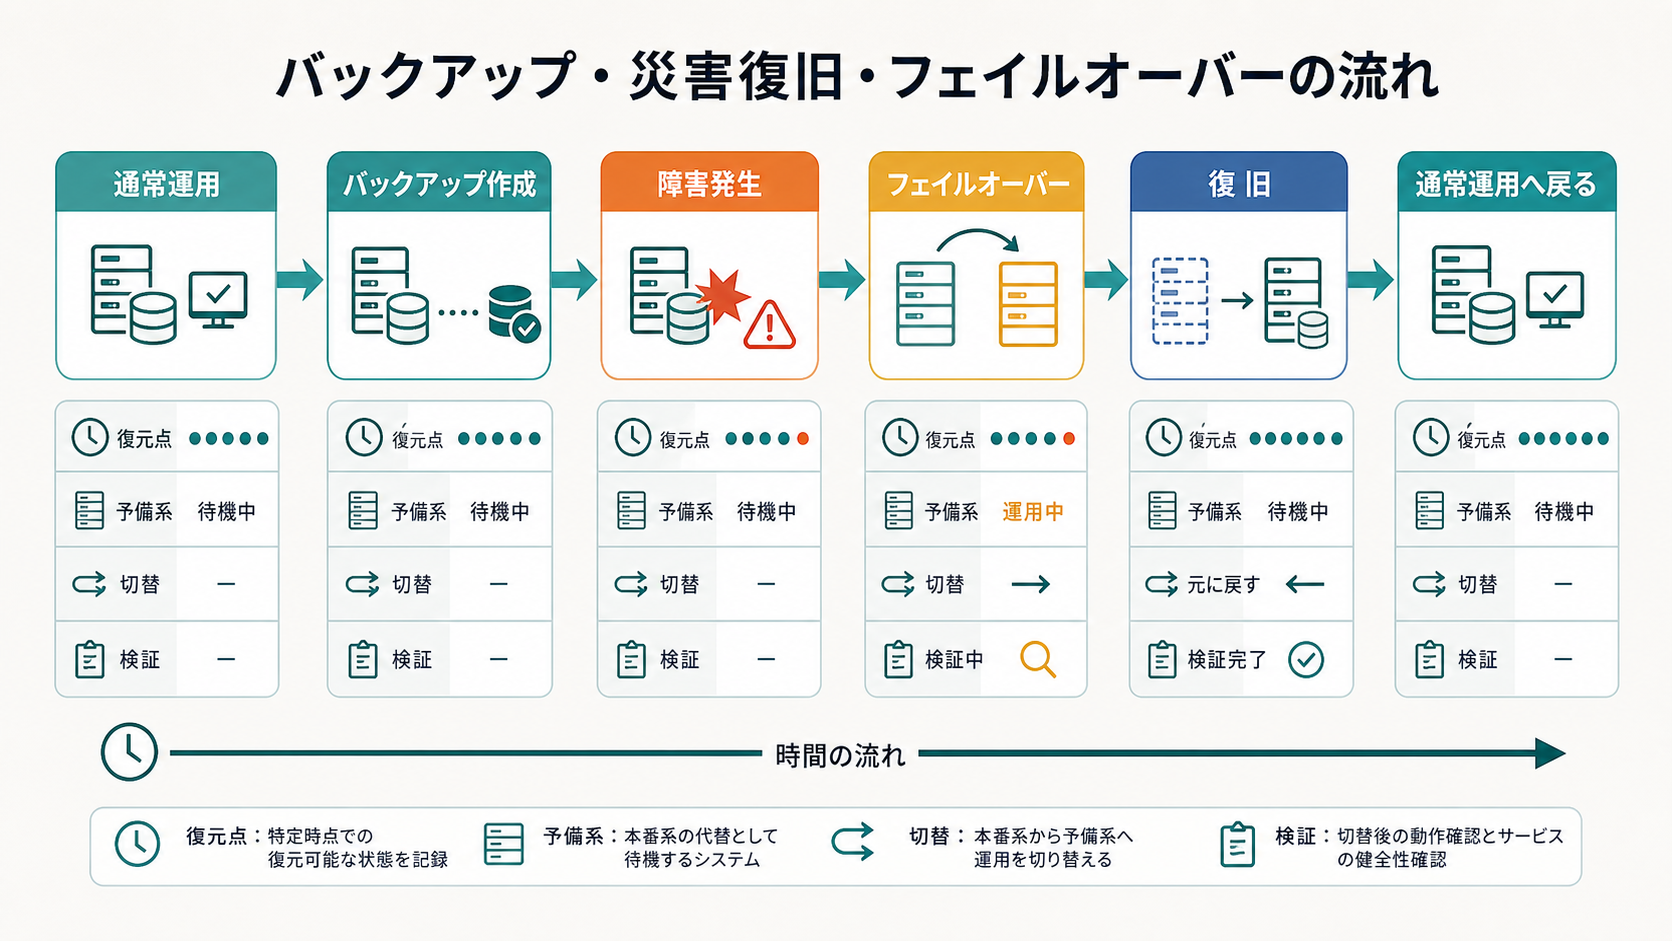
\includegraphics[width=0.96\linewidth]{assets/generated_figures/ch06/fig-ch06-05.png}}{\fbox{\parbox[c][48mm][c]{0.9\linewidth}{\centering 画像生成待ち\\バックアップ・災害復旧・フェイルオーバーの流れ}}}
\caption{バックアップ・災害復旧・フェイルオーバーの流れ}
\label{fig:ch06-05}
\end{figure}
